% !TEX program = xelatex
\documentclass[11pt,a4paper]{article}

\usepackage[a4paper,margin=2.2cm]{geometry}
\usepackage{fontspec}
\usepackage{graphicx}
\usepackage{booktabs}
\usepackage{tabularx}
\usepackage{array}
\usepackage{float}
\usepackage{xcolor}
\usepackage{hyperref}
\usepackage{enumitem}
\usepackage{caption}
\usepackage{subcaption}
\usepackage{longtable}
\usepackage{listings}

\IfFontExistsTF{TeX Gyre Termes}{
    \setmainfont{TeX Gyre Termes}
}{
    \IfFontExistsTF{Times New Roman}{
        \setmainfont{Times New Roman}
    }{
        \setmainfont{Latin Modern Roman}
    }
}
\IfFontExistsTF{TeX Gyre Heros}{
    \setsansfont{TeX Gyre Heros}
}{
    \setsansfont{Arial}
}
\IfFontExistsTF{Latin Modern Mono}{
    \setmonofont[Scale=0.90]{Latin Modern Mono}
}{
    \setmonofont[Scale=0.86]{Menlo}
}

\hypersetup{
    colorlinks=true,
    linkcolor=blue,
    citecolor=blue,
    urlcolor=blue
}

\setlist[itemize]{leftmargin=1.45em}
\setlist[enumerate]{leftmargin=1.45em}
\renewcommand{\arraystretch}{1.14}
\newcolumntype{Y}{>{\raggedright\arraybackslash}X}
\newcolumntype{Z}{>{\raggedright\arraybackslash\ttfamily\footnotesize}X}
\emergencystretch=3em

\lstset{
    basicstyle=\ttfamily\small,
    breaklines=true,
    frame=single,
    columns=fullflexible
}

\renewcommand{\texttt}[1]{{\small\ttfamily\textcolor{black!85}{#1}}}
\newcommand{\idx}[1]{\texttt{#1}}
\newcommand{\idxsplit}[2]{\begin{tabular}[t]{@{}l@{}}\texttt{#1}\\\texttt{#2}\end{tabular}}

\title{\textbf{Cost-of-Living Data Platform}\\
\large Cloud Data Pipeline, Search Taxonomy, and Analytics API}
\author{Tzz and Contributors}
\date{2026}

\begin{document}

\maketitle

\begin{abstract}
The cost-of-living data platform monitors Australian public discussion, media coverage, and official CPI indicators through a cloud data pipeline. It collects public records from Bluesky, Mastodon, and GDELT GKG archive files; normalises source-specific records into a unified raw schema; processes text into topics, sentiment labels, and quality flags; and serves chart-ready analytics through a FastAPI REST API. The public architecture keeps one API serving path, uses Fission for scheduled data collection, runs NLP processing through KEDA-scaled Kubernetes workers, and stores data in Elasticsearch with ILM-managed processed indices.
\end{abstract}

\tableofcontents
\newpage

\section{Product Scope}

Cost-of-living pressure appears in household expenses such as rent, groceries, energy, fuel, healthcare, education, and debt. Official indicators provide stable monthly context, while public social and media records provide timely but noisy signals. The platform focuses on repeatable monitoring rather than causal inference:

\begin{itemize}
    \item collect public source records on schedules;
    \item filter for Australian context and cost-of-living relevance;
    \item preserve source provenance and raw processing state;
    \item process records into topics, sentiment, and quality flags;
    \item expose REST endpoints for notebooks, dashboards, and operational checks;
    \item compare selected discussion patterns with official CPI observations.
\end{itemize}

The main analytical constraint is representativeness. Bluesky and Mastodon show public platform discussion, GDELT shows media coverage, and CPI shows official price movement. These sources should be compared, not collapsed into one sentiment score.

\section{Data Sources and Taxonomy}

\begin{table}[H]
\centering
\caption{Source roles}
\begin{tabularx}{\linewidth}{p{0.18\linewidth}p{0.23\linewidth}Y}
\toprule
Source & Role & Interpretation \\
\midrule
Bluesky & Public social discussion & Short public posts with search-based collection and Australian context filtering. \\
Mastodon & Public social discussion & Public posts from multiple instances, useful as a second social signal. \\
GDELT GKG & Media coverage & Archive-based media records, treated as attention in news coverage rather than direct public sentiment. \\
ABS CPI & Official indicator & Monthly official comparison signal for selected consumer categories. \\
\bottomrule
\end{tabularx}
\end{table}

The taxonomy lives in \idx{data/cost\_of\_living\_keywords.csv}. It covers housing, groceries, energy, fuel, transport, eating out, healthcare, home goods, education, inflation, wages, and debt. Terms were selected from common Australian spending categories, CPI-aligned categories, and locally meaningful terms such as supermarket brands, public transport references, and healthcare language.

GDELT uses the public GKG master file list rather than rate-limited article search. Incremental harvesting and historical backfill share the same archive processor: read list metadata, download \idx{.gkg.csv.zip} archives, verify checksums, extract CSV rows, filter for Australian cost-of-living records, and bulk index matching records.

\section{Cloud Architecture}

\begin{figure}[H]
\centering
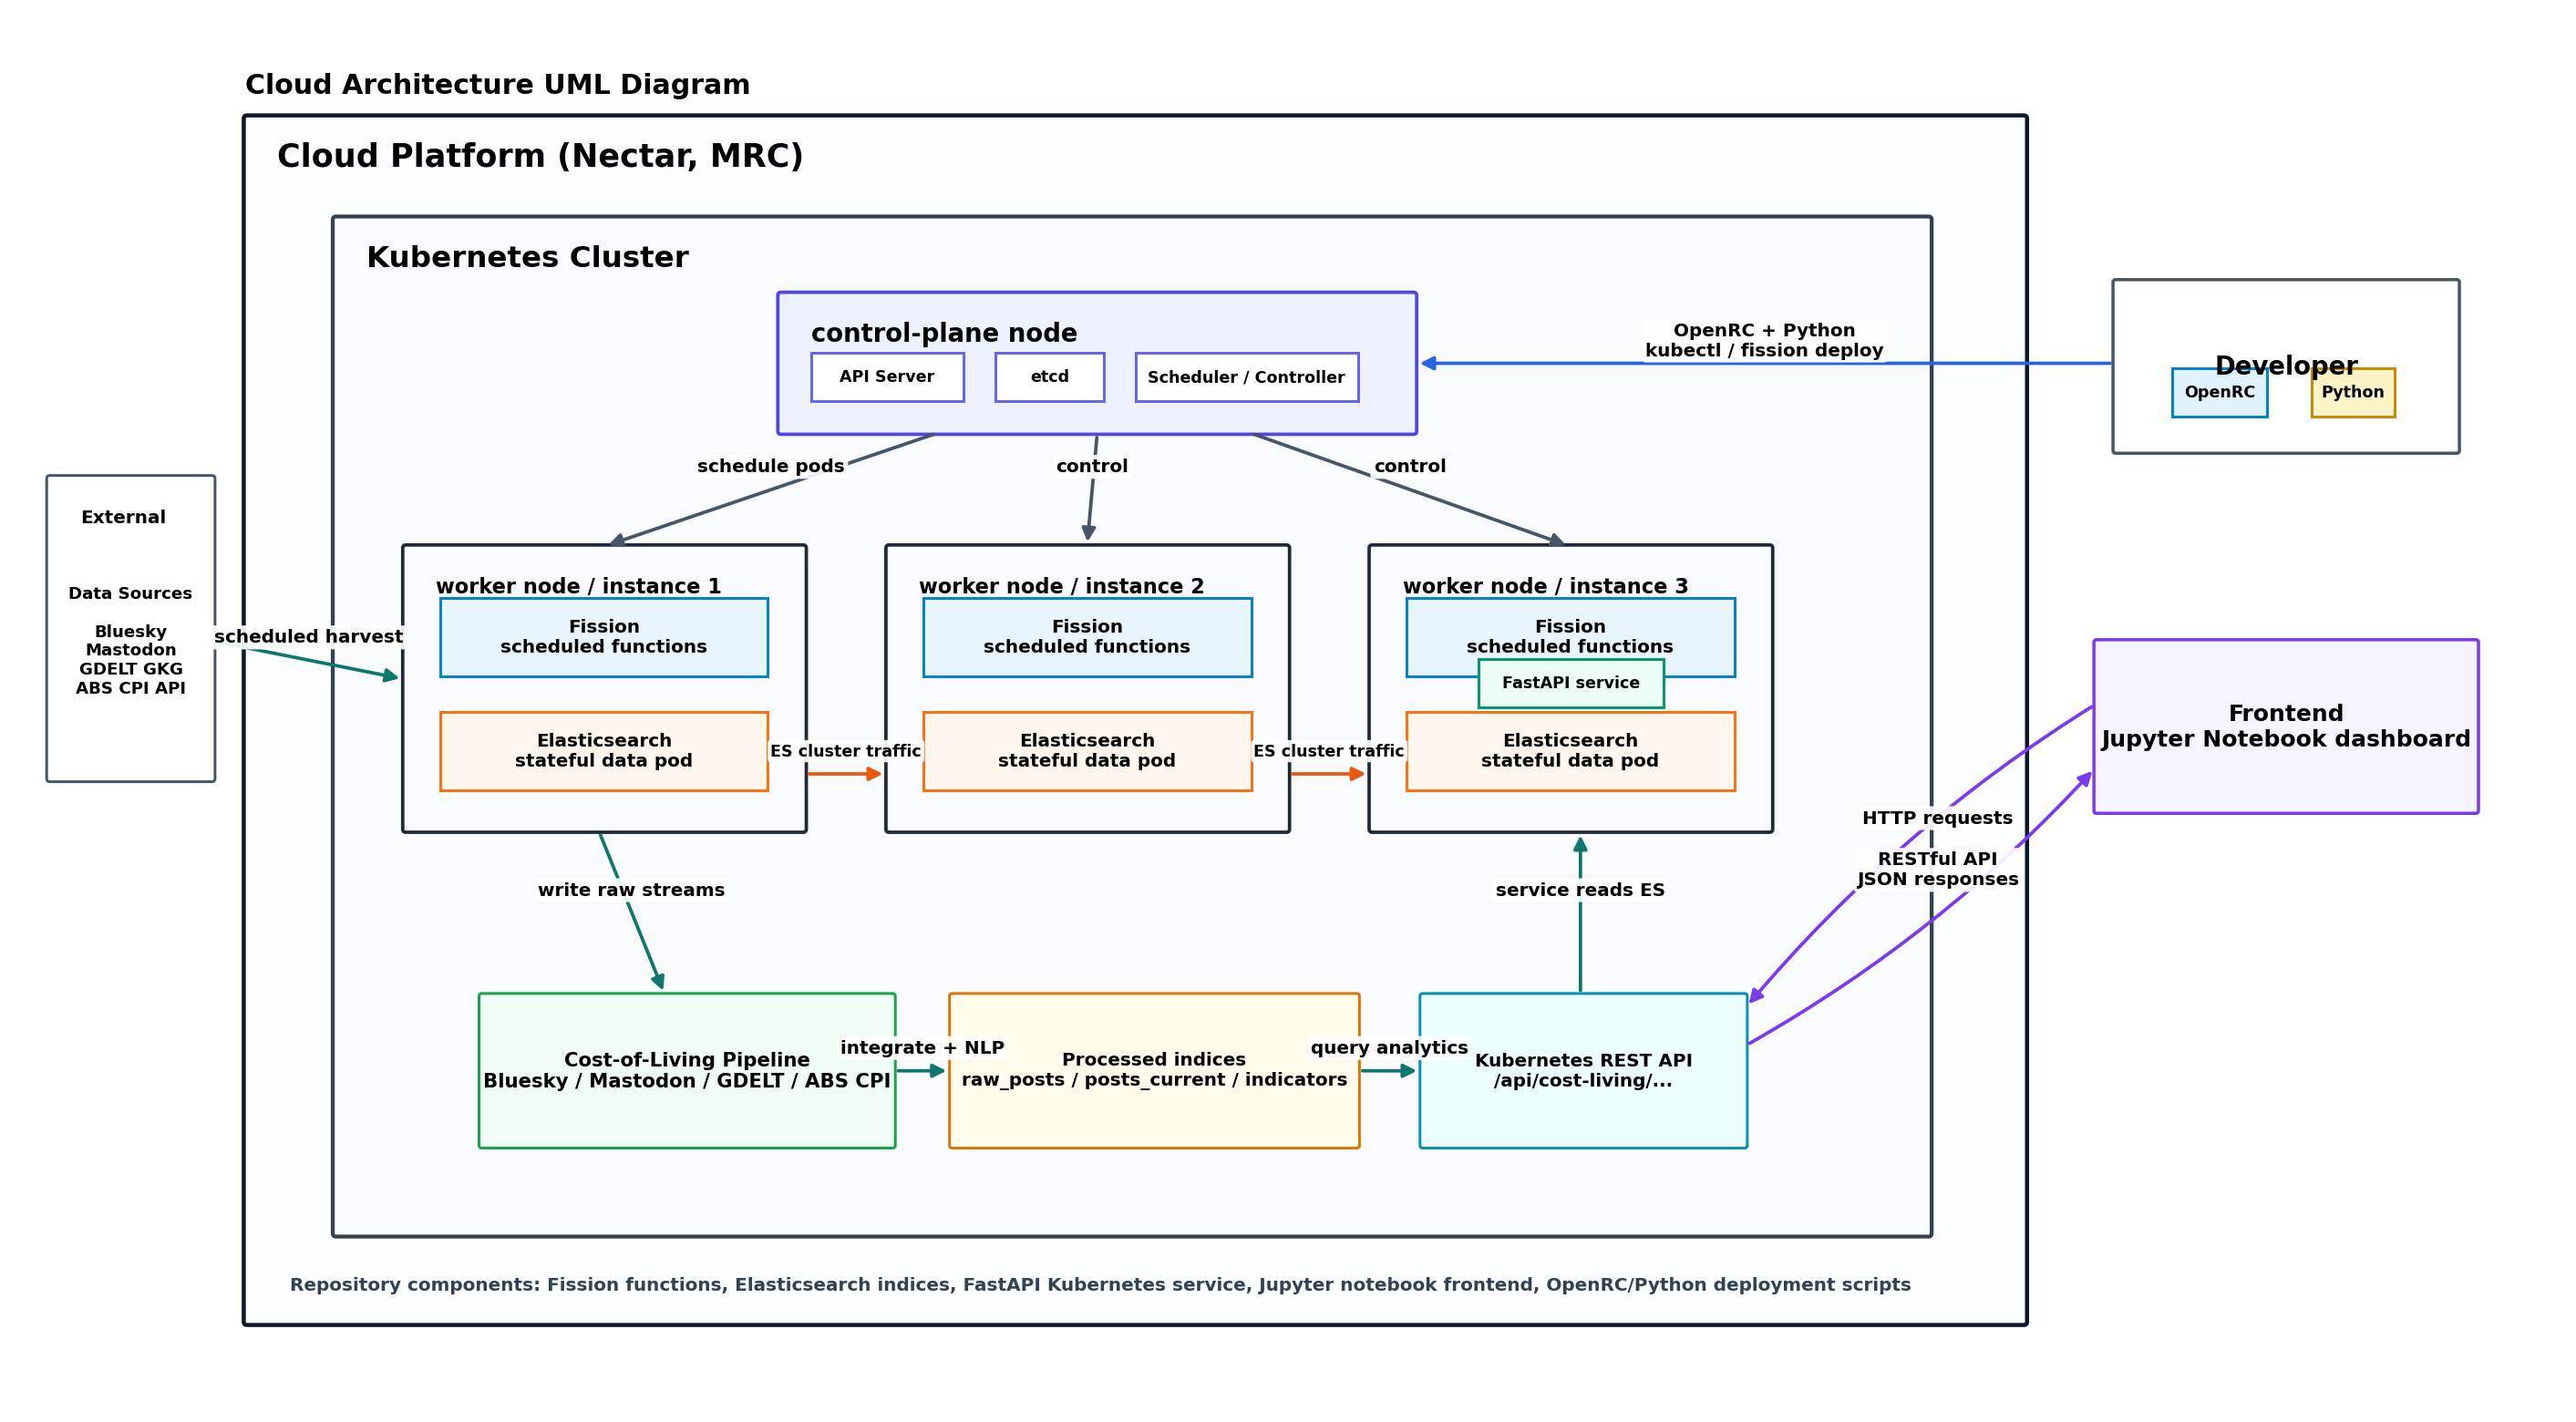
\includegraphics[width=\linewidth]{../evidence/architecture_diagram.png}
\caption{Pipeline architecture}
\label{fig:architecture}
\end{figure}

The platform is organised around one public API path and several scheduled pipeline jobs. FastAPI serves analytics and operational endpoints under \idx{/api/cost-living}. Fission runs scheduled harvesters, raw integration, and official indicator collection. Redis stores runtime locks, recent lifecycle events, short-lived API cache entries, and the NLP work queue. KEDA watches the Redis queue and scales NLP workers from zero. Elasticsearch stores raw records, processed records, CPI observations, and queryable processing status.

\begin{table}[H]
\centering
\caption{Runtime components}
\begin{tabularx}{\linewidth}{p{0.24\linewidth}Y}
\toprule
Component & Responsibility \\
\midrule
Fission harvesters & Collect Bluesky, Mastodon, GDELT, and CPI records on schedules. \\
Raw integrator & Convert platform streams into the unified raw schema and enqueue NLP work. \\
KEDA NLP worker & Consume Redis work items, claim pending raw records, clean text, classify topics, score sentiment, and write processed records. \\
FastAPI API & Provide analytics, health, cache, rate-limit, queue, and pipeline endpoints. \\
Redis & Coordinate locks, lifecycle events, shared API cache, active queue, and dead-letter queue. \\
Elasticsearch & Store raw streams, unified raw state, processed analytics, CPI indicators, and monthly rollups. \\
\bottomrule
\end{tabularx}
\end{table}

\begin{figure}[H]
\centering
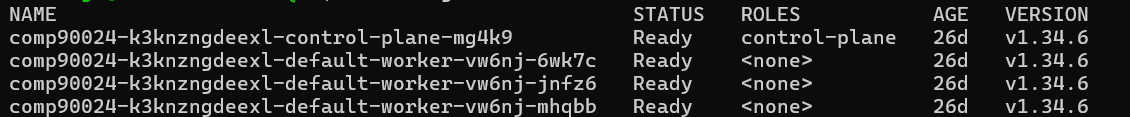
\includegraphics[width=0.9\linewidth]{../evidence/kubernetes_nodes.png}
\caption{Kubernetes node layout}
\label{fig:kubernetes-nodes}
\end{figure}

\begin{figure}[H]
\centering
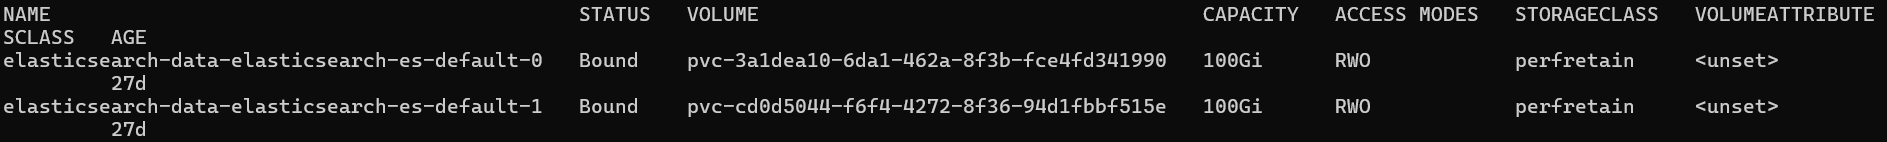
\includegraphics[width=\linewidth]{../evidence/elasticsearch_pvc_claims.png}
\caption{Elasticsearch persistent volume claims}
\label{fig:elasticsearch-pvc}
\end{figure}

\section{Elasticsearch and Queue Design}

\begin{table}[H]
\centering
\caption{Main indices and aliases}
\begin{tabularx}{\linewidth}{p{0.34\linewidth}p{0.28\linewidth}Y}
\toprule
Index or alias & Writer & Reader \\
\midrule
\idxsplit{cost\_living\_bluesky}{raw\_stream} & Bluesky harvester & Raw integrator \\
\idxsplit{cost\_living\_mastodon}{raw\_stream} & Mastodon harvesters & Raw integrator \\
\idxsplit{cost\_living\_gdelt}{raw\_stream} & GDELT harvester & Raw integrator \\
\idx{cost\_living\_raw\_posts} & Raw integrator & NLP worker, status API \\
\idxsplit{cost\_living\_processed}{posts\_write} & NLP worker & Elasticsearch rollover \\
\idxsplit{cost\_living\_processed}{posts-*} & Write alias & API through read alias \\
\idx{cost\_living\_posts\_current} & Alias update & Analytics API \\
\idx{cost\_living\_indicators} & CPI harvester & Comparison API \\
\idxsplit{cost\_living\_monthly}{topic\_metrics} & Rollup job & Optional API acceleration \\
\bottomrule
\end{tabularx}
\end{table}

Raw and processed records are separate. Raw records retain source provenance, source identifiers, original text, timestamps, and processing status. Processed records hold topic labels, sentiment, quality flags, and chart-ready fields. The API reads processed data through \idx{cost\_living\_posts\_current}, while the worker writes through \idx{cost\_living\_processed\_posts\_write}. The processed backing indices use Elasticsearch ILM and rollover, so frontend routes remain stable while storage evolves.

Processing state is explicit. A raw record starts as \idx{pending}, a worker atomically moves it to \idx{processing}, and the final state becomes \idx{processed}, \idx{discarded}, or \idx{error}. Stale \idx{processing} records can be reclaimed after a configured timeout.

Redis handles runtime concerns that do not belong in Elasticsearch. The active NLP queue is:

\begin{lstlisting}
cost_living_pipeline:queue:nlp
\end{lstlisting}

Messages have a bounded retry budget. Transient failures are requeued with attempt metadata and the latest error. Messages that exceed \idx{NLP\_QUEUE\_MAX\_ATTEMPTS}, cannot be decoded, or use an unsupported message kind are isolated in:

\begin{lstlisting}
cost_living_pipeline:queue:nlp:dead-letter
\end{lstlisting}

The queue status endpoint reports both active queue depth and dead-letter depth, so worker failures are visible instead of silently looping.

\section{API and Operations}

The API is read-only for analytics and exposes operational endpoints for cloud checks:

\begin{table}[H]
\centering
\caption{Endpoint groups}
\begin{tabularx}{\linewidth}{p{0.34\linewidth}Y}
\toprule
Endpoint group & Purpose \\
\midrule
\idx{/health} & API and Elasticsearch readiness. \\
\idx{/overview}, \idx{/topics}, \idx{/sentiment} & High-level counts, topic distribution, and sentiment summaries. \\
\idx{/trends/*} & Daily and monthly time-series views. \\
\idx{/platforms/*} & Source comparison and plugin metadata. \\
\idx{/cpi/*} & Official CPI comparison endpoints. \\
\idx{/data-quality/*} & Quality flag and clean-vs-all comparisons. \\
\idx{/pipeline/*} & Processing status, runtime events, and queue depths. \\
\idx{/cache/status} & Redis or in-memory API cache diagnostics. \\
\idx{/rate-limit/status} & API rate-limit configuration and backend. \\
\idx{/metrics} & Prometheus request, latency, cache, queue, and rate-limit metrics. \\
\bottomrule
\end{tabularx}
\end{table}

Every request receives an \idx{X-Request-ID}. Incoming IDs are preserved when supplied by clients, and generated IDs are attached to structured API logs. OpenTelemetry spans can be emitted through the configured exporter, and Prometheus metrics are exposed for scraping.

\section{Validation Evidence}

The current repository validation passes:

\begin{lstlisting}[language=bash]
63 passed
Public release check passed for 122 release files.
\end{lstlisting}

Cloud smoke validation covered the public API prefix, queue status, rate-limit status, request-id propagation, Prometheus metrics, KEDA worker scaling, and processed-index writes through the rollover alias.

\begin{table}[H]
\centering
\caption{Operational validation}
\begin{tabularx}{0.82\linewidth}{p{0.38\linewidth}Y}
\toprule
Check & Result \\
\midrule
API smoke test & 25 endpoints passed. \\
Request tracing & \idx{X-Request-ID} preserved in responses and logs. \\
Rate limiting & Redis-backed status endpoint available. \\
Prometheus metrics & Request, latency, cache, queue, and rate-limit metrics exposed. \\
KEDA worker & Scaled from zero, processed queue work, and scaled back down. \\
Elasticsearch ILM & Processed write and read aliases verified. \\
Public release check & Sensitive local markers and notebook outputs cleared. \\
\bottomrule
\end{tabularx}
\end{table}

\section{Analytics Results}

\subsection{Processing Outcomes}

\begin{figure}[H]
\centering
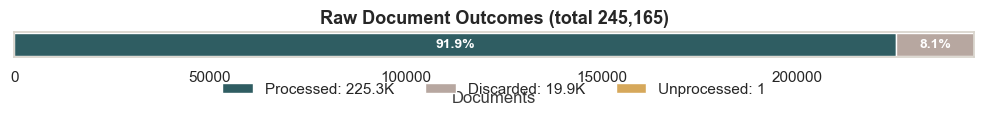
\includegraphics[width=0.95\linewidth]{../evidence/raw_document_outcomes.png}
\caption{Raw document processing outcomes}
\label{fig:raw-outcomes}
\end{figure}

The processed corpus contains a large majority of usable records, with discarded records retained as visible processing outcomes instead of being deleted. This makes the pipeline auditable: filtering decisions can be checked through raw status fields and API diagnostics.

\begin{figure}[H]
\centering
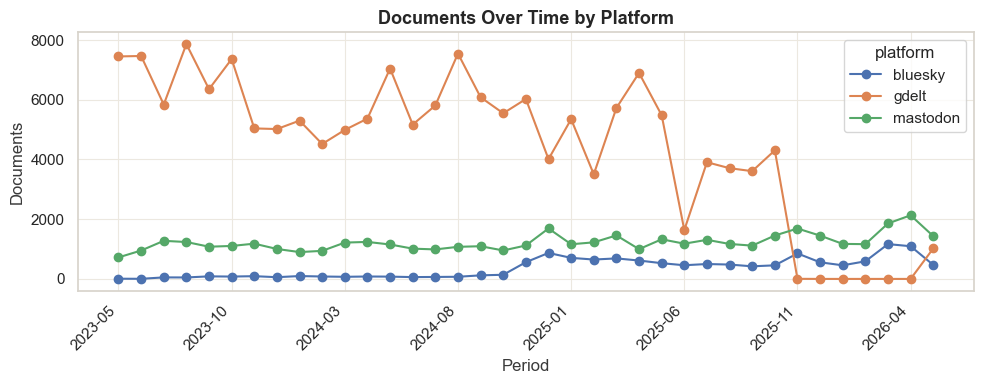
\includegraphics[width=0.95\linewidth]{../evidence/documents_over_time_by_platform.png}
\caption{Documents over time by platform}
\label{fig:documents-over-time}
\end{figure}

Volume differs by source. Social sources are useful for personal and topical discussion, while GDELT is better interpreted as media attention. Keeping source groups explicit avoids mixing signals with different meanings.

\subsection{Sentiment and Topic Patterns}

\begin{figure}[H]
\centering
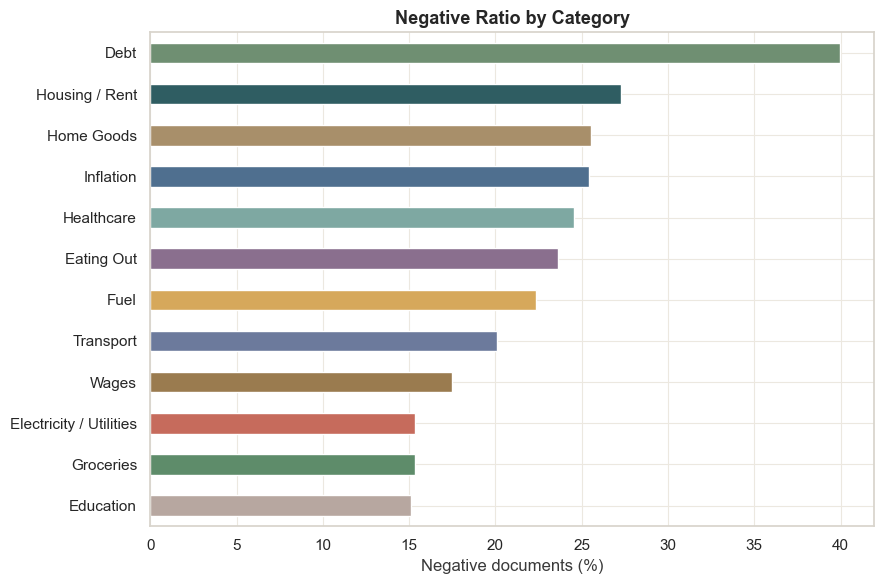
\includegraphics[width=0.82\linewidth]{../evidence/negative_ratio_by_category.png}
\caption{Negative ratio by cost-of-living category}
\label{fig:negative-ratio}
\end{figure}

\begin{figure}[H]
\centering
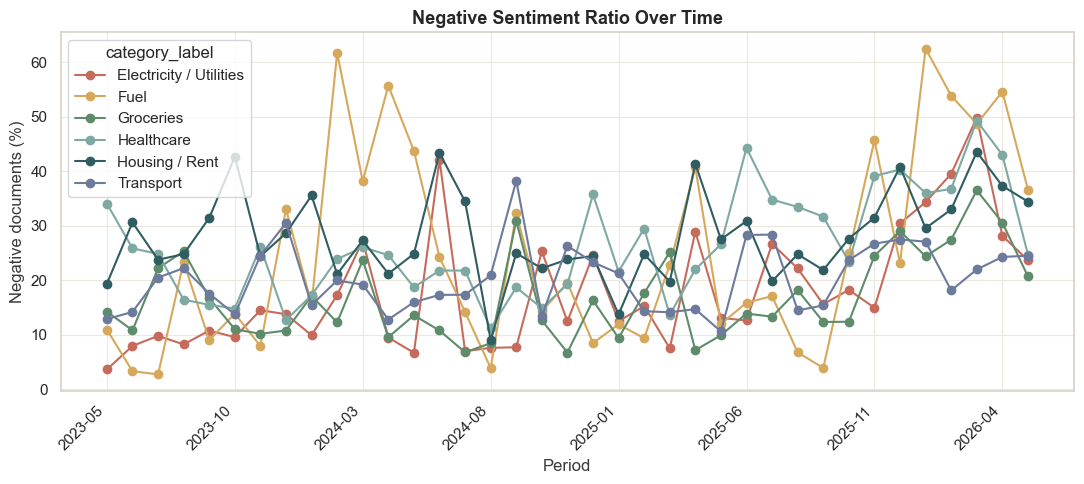
\includegraphics[width=0.95\linewidth]{../evidence/negative_sentiment_trend.png}
\caption{Negative sentiment trend}
\label{fig:negative-trend}
\end{figure}

Negative sentiment is concentrated in categories where household budgets are directly affected, such as housing, groceries, energy, and transport. Trend charts are more useful when combined with source filters because platform volume and media coverage can change independently.

\begin{figure}[H]
\centering
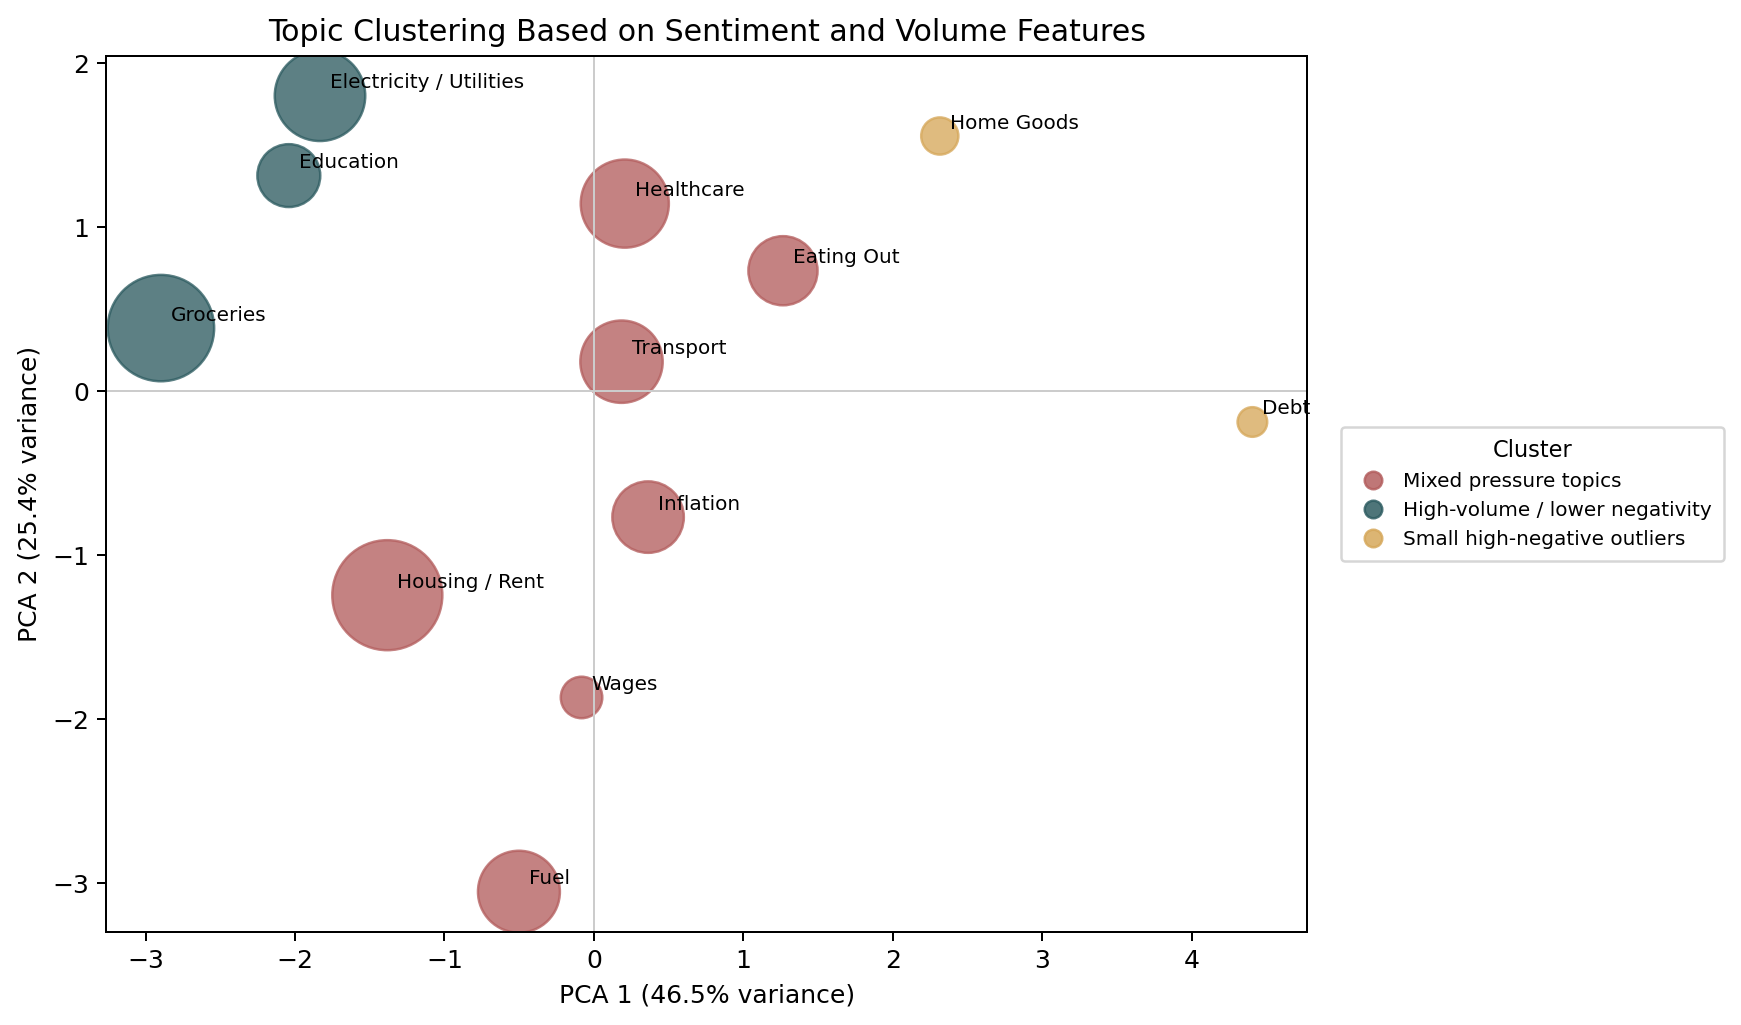
\includegraphics[width=0.86\linewidth]{../evidence/topic_clustering_pca.png}
\caption{Topic clustering PCA}
\label{fig:topic-pca}
\end{figure}

\begin{figure}[H]
\centering
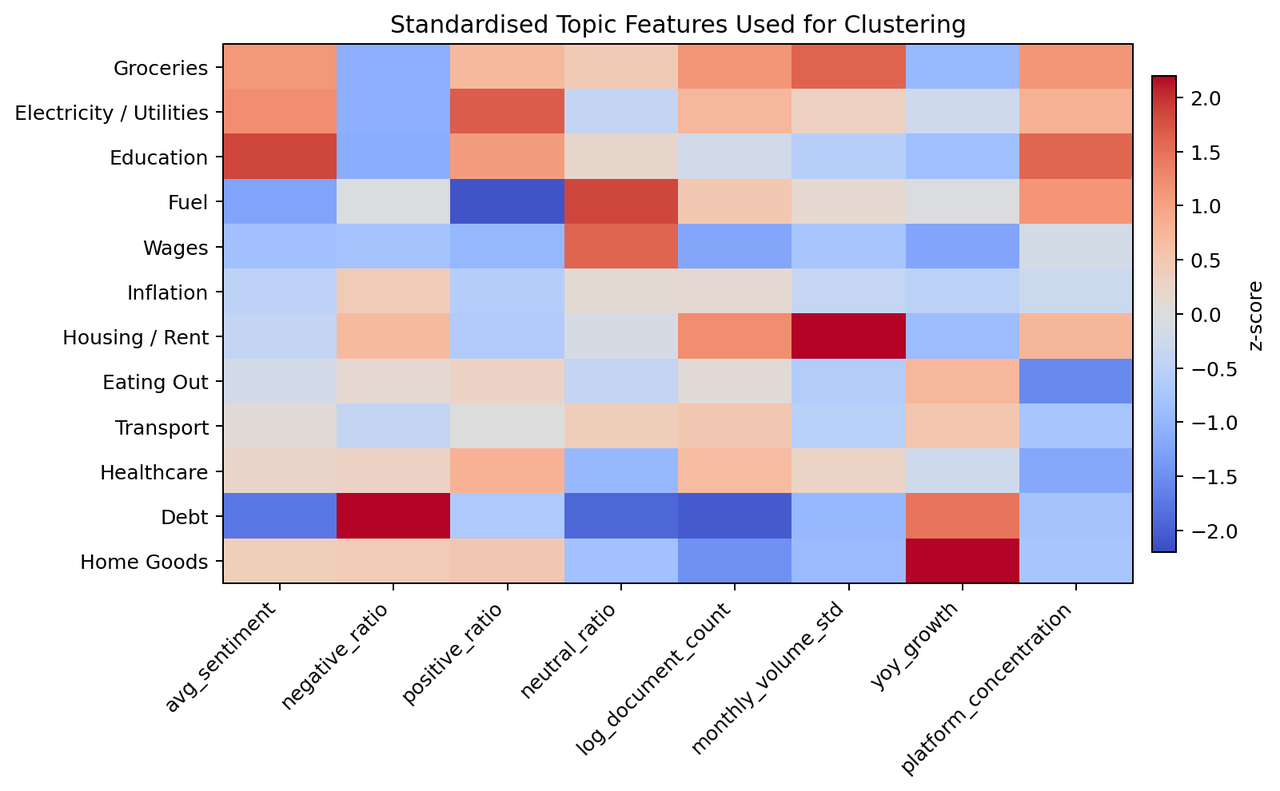
\includegraphics[width=0.82\linewidth]{../evidence/topic_clustering_feature_heatmap.png}
\caption{Topic clustering feature heatmap}
\label{fig:topic-feature-heatmap}
\end{figure}

Topic features show overlap between cost categories. Rent, groceries, fuel, energy, and inflation can appear in the same posts, so rule-based topic labelling should be interpreted as a practical monitoring label rather than a complete semantic model.

\subsection{Platform Differences}

\begin{figure}[H]
\centering
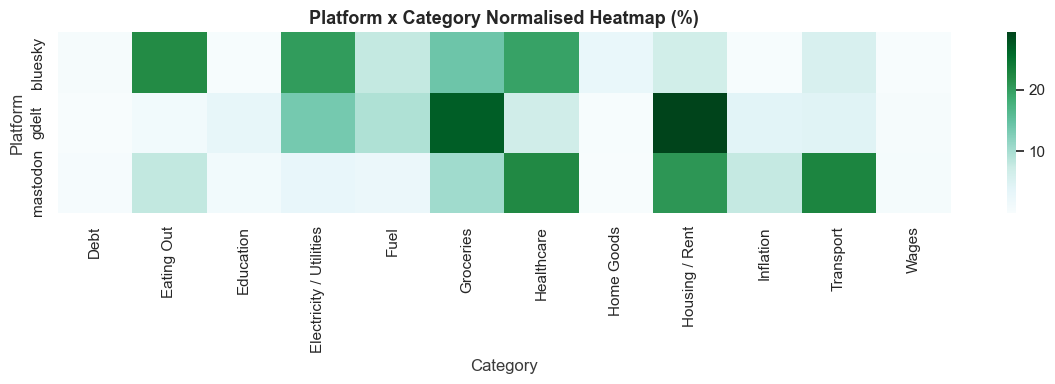
\includegraphics[width=0.95\linewidth]{../evidence/platform_category_normalised_heatmap.png}
\caption{Normalised category distribution by platform}
\label{fig:platform-category}
\end{figure}

\begin{figure}[H]
\centering
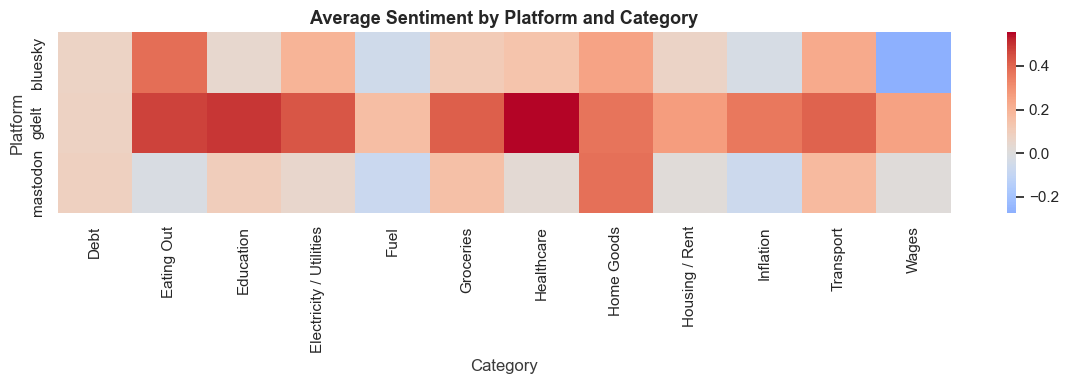
\includegraphics[width=0.95\linewidth]{../evidence/platform_category_sentiment_heatmap.png}
\caption{Platform and category sentiment heatmap}
\label{fig:platform-sentiment}
\end{figure}

Platform-level comparisons are most useful for understanding source bias. Bluesky and Mastodon reflect public social posting behaviour, while GDELT reflects coverage in media records. The API therefore exposes \idx{source\_group} and \idx{platform} filters on relevant analytics routes.

\subsection{CPI Comparison}

\begin{figure}[H]
\centering
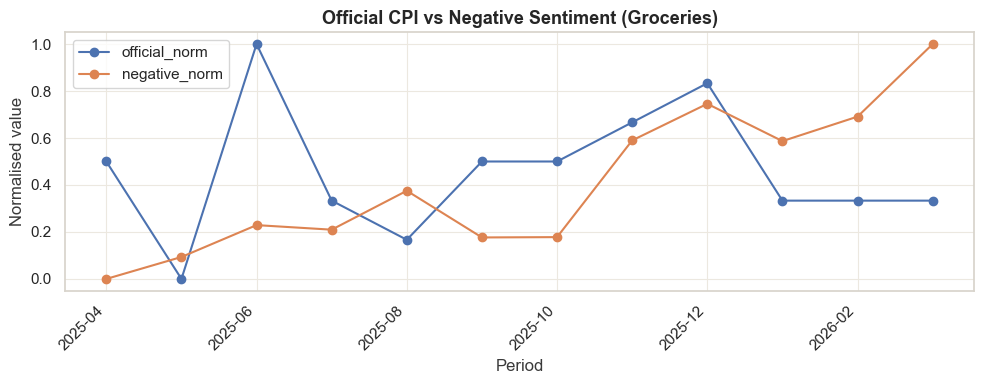
\includegraphics[width=0.9\linewidth]{../evidence/cpi_groceries_comparison.png}
\caption{Grocery discussion compared with CPI}
\label{fig:cpi-groceries}
\end{figure}

\begin{figure}[H]
\centering
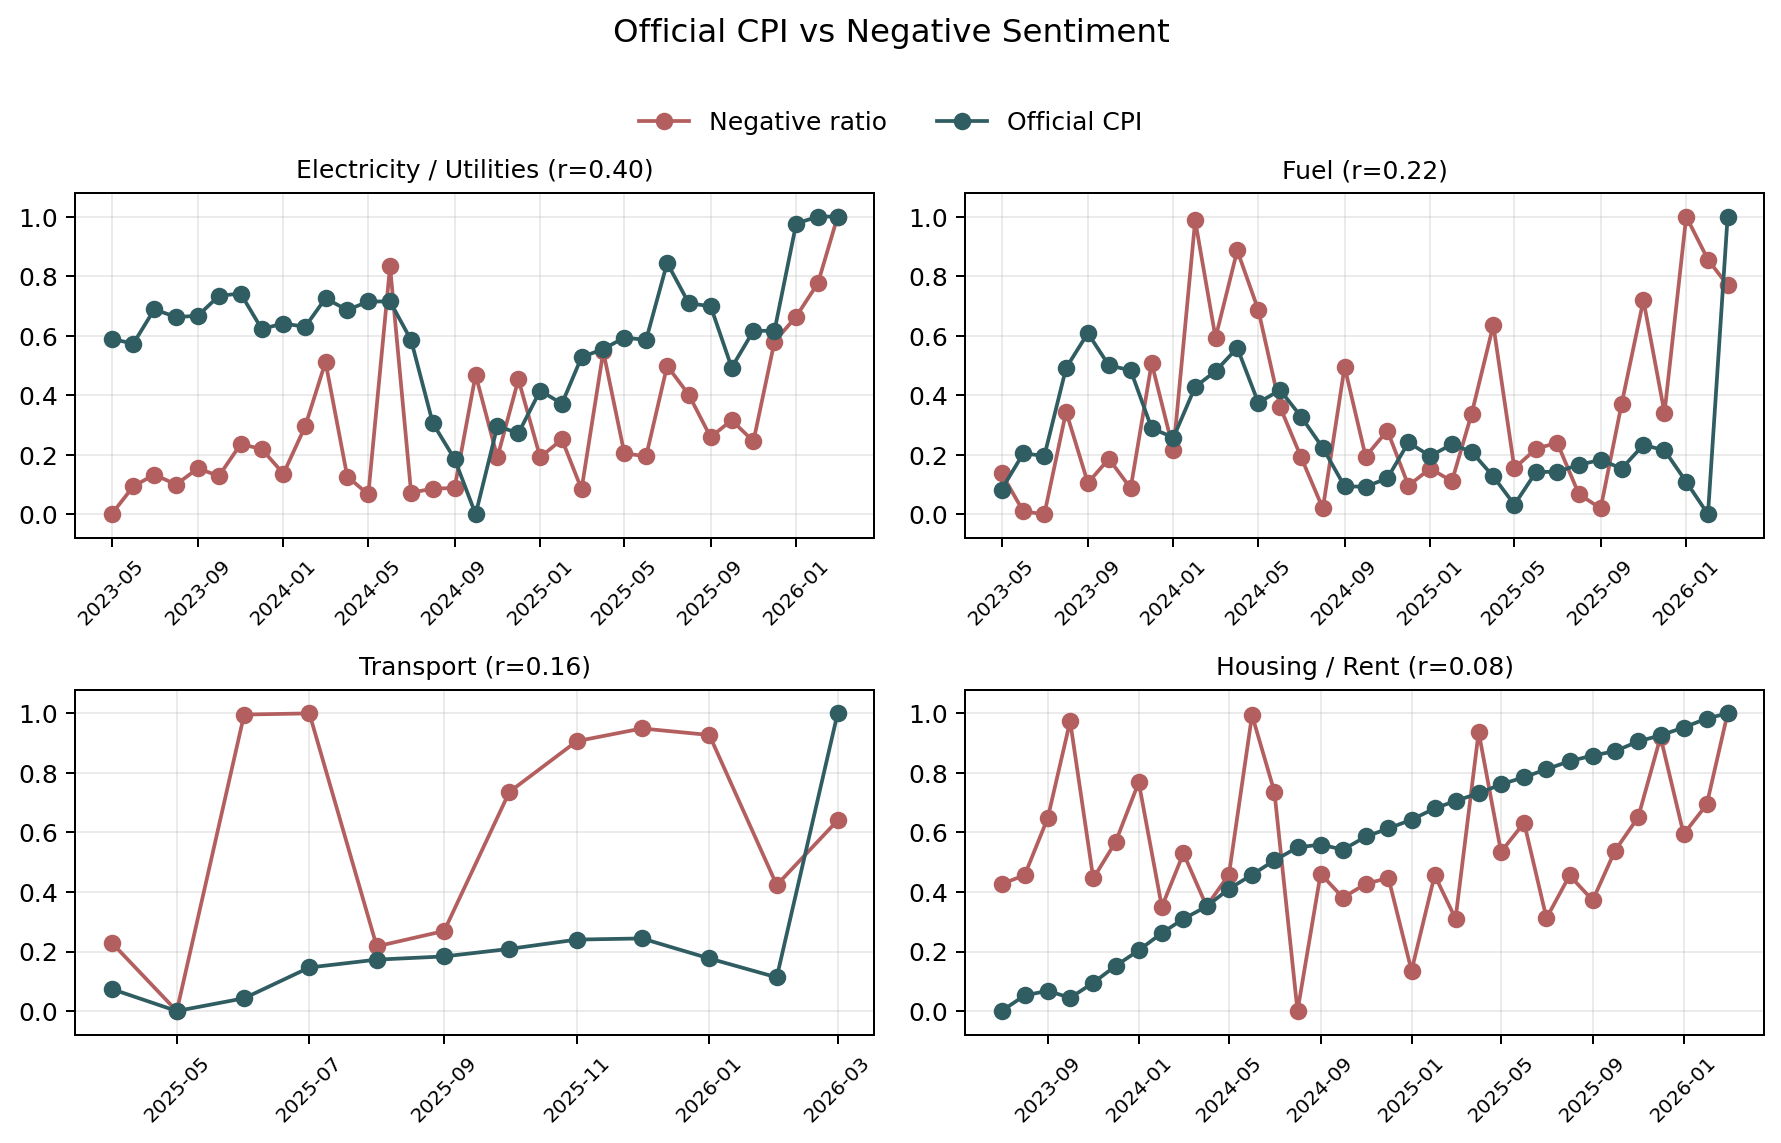
\includegraphics[width=0.95\linewidth]{../evidence/cpi_sentiment_comparison_grid.png}
\caption{CPI and sentiment comparison grid}
\label{fig:cpi-grid}
\end{figure}

CPI comparison gives official context but does not prove causation. CPI is monthly and lagged, while social and media records respond to events, platform behaviour, and collection windows. The comparison is best used as a contextual signal for dashboard exploration.

\section{Reliability and Limitations}

\begin{longtable}{p{0.22\linewidth}p{0.34\linewidth}p{0.34\linewidth}}
\caption{Reliability mechanisms}\\
\toprule
Area & Risk & Handling \\
\midrule
\endfirsthead
\toprule
Area & Risk & Handling \\
\midrule
\endhead
Duplicate records & Overlapping harvest windows or repeated keywords. & Stable source IDs, URLs, document IDs, and Elasticsearch upserts. \\
External APIs & Rate limits, timeouts, or temporary failures. & Source-specific retries, state checkpoints, and later scheduled recovery. \\
Raw integration & Different platform schemas. & Unified raw contract with source index and source document identifiers. \\
NLP processing & Worker crashes or bad messages. & Atomic claiming, stale retry, Redis retry budget, and dead-letter queue. \\
API usage & Expensive repeated dashboard reads. & Short shared cache TTL, rate limiting, and request-level tracing. \\
Elasticsearch growth & Processed index expansion. & ILM-managed write alias and stable read alias. \\
\bottomrule
\end{longtable}

The main limitations remain analytical. Public social platforms are not representative of all Australians. GDELT is media coverage, not public sentiment. Keyword taxonomy is transparent and auditable, but it can miss context and cross-topic meaning. VADER is lightweight and interpretable, but it can misread sarcasm, slang, political language, quoted text, and metadata-heavy records. City-level analysis is intentionally excluded because source records do not provide reliable city fields.

\section{Conclusion}

The platform demonstrates a maintainable pattern for cloud-based public text monitoring: source-specific ingestion, unified raw state, queued NLP processing, explicit data contracts, operational API endpoints, and Elasticsearch-backed analytics. The strongest engineering choices are the single API serving path, archive-based GDELT ingestion, Redis-backed runtime diagnostics and worker queueing, KEDA scaling, dead-letter isolation, ILM-managed processed indices, request-level tracing, rate limiting, and a testable FastAPI interface.

Future work should focus on end-to-end container integration tests, API contract tests from the OpenAPI schema, managed dashboard manifests for Prometheus and Grafana, raw-stream lifecycle policies, and a repeatable load-test baseline.

\newpage
\nocite{abs_api,gdelt,bluesky_api,mastodon_api,kubernetes_docs,fission_docs,elasticsearch_docs,vader}
\bibliographystyle{plain}
\bibliography{references}

\end{document}
